\chapter{Grundlagen}

Quelle 1: Access Points Service Set Identifier (SSID) for Localization and Tracking
Quelle 2: RSSI-Based Indoor Localization With the Internet of Things
Quelle 3: Survey on Indoor localization System and Recent Advances of WIFI Fingerprinting Technique

\section{WiFi-Fingerprinting}

Gute Grundlagenquelle: Overview of WiFi fingerprinting-based indoor positioning -> Was ist Indoor Ortung, was gibt es für Möglichkeiten, Offline/Online Phase, was für Modelle gibt es?

\section{Indoor-Ortung: Offline- und Online-Phase}
\section{SSID, BSSID und RSSI}


\subsection{SSID}

Der Service Set Identifier (SSID) ist ein eindeutiger Bezeichner, der ein drahtloses Netzwerk kennzeichnet. SSIDs sind alphanumerische Zeichenfolgen, die vom Netzwerkadministrator festgelegt werden. Die SSID ermöglicht es Nutzern, zwischen verschiedenen WiFi-Netzwerken zu unterscheiden und das gewünschte Netzwerk auszuwählen. In einem Indoor-Lokalisierungsszenario kann die SSID als Landmarke für Access Points genutzt werden, um die Position eines Benutzers zu bestimmen (Quelle 1, Kapitel 1, Seite 5460).

\subsection{BSSID}

Der Basic Service Set Identifier (BSSID) ist eine eindeutige Kennung für jeden Access Point innerhalb eines WiFi-Netzwerks. Diese Kennung besteht aus der MAC-Adresse des Access Points, die fest zugewiesen und unveränderlich ist. In Netzwerken mit mehreren Access Points, die dieselbe SSID nutzen, ermöglicht die BSSID die genaue Unterscheidung der einzelnen Access Points. Dies ist besonders wichtig für die Lokalisierung und Netzwerkverwaltung, da es die Identifikation und Verfolgung spezifischer Access Points ermöglicht (Quelle 1, Kapitel 1, Seite 5460).

\subsection{RSSI}

Der Received Signal Strength Indicator (RSSI) ist ein Maß für die Stärke des empfangenen WiFi-Signals an einem bestimmten Punkt. RSSI-Werte werden von der Netzwerkkarte des Geräts gemessen und in der App aufgezeichnet. Diese Werte spielen eine entscheidende Rolle bei der Erstellung von Fingerprints für die Indoor-Lokalisierung, da die Signalstärke als Indikator für die Entfernung zwischen dem Gerät und dem Access Point genutzt wird. Schwächere RSSI-Werte deuten dabei auf eine größere Entfernung hin (Quelle 1, Kapitel 1, Seite 5464).

\section{Verhalten von RSSI-Werten in Bezug auf Entfernung}

Quelle 2:

Die RSSI-Werte nehmen mit zunehmender Distanz zwischen Sender und Empfänger ab, und können mit dem Pfadverlustmodell beschrieben werden. Das Pfadverlustmodell beschreibt den Zusammenhang zwischen der Entfernung und der Signalstärke, und wird durch die folgende Gleichung dargestellt:

\begin{equation}
    RSSI = -10n \log_{10}(d) + C
\end{equation}

wobei n der Pfadverlustexponent ist, der je nach Umgebung variiert, d die Distanz zwischen Sender und Empfänger ist und A der RSSI-Wert in einem Meter Entfernung vom Sender ist.

Umgebung der Quelle: Im Raum sind viele Computer und eine große Anzahl an WiFi- und BLE-Geräten, Ein Forschungslabor mit den Abmessungen 10,8 m x 7,3 m.

Ergebnisse: n = 2.013, C = -49,99 dBm

Die Path-Loss-Modell-Gleichung mit den Parametern \(n = 2.013\) und \(C = -49.99\) ist:

In Abbildung \ref{fig:rssi_distance} ist der Zusammenhang zwischen RSSI und Entfernung dargestellt. Dieser Abschnitt dient dazu um eine Vorstellung davon zu bekommen, wie sich RSSI-Werte in Bezug auf die Entfernung verhalten.

\begin{figure}[h]
    \centering
    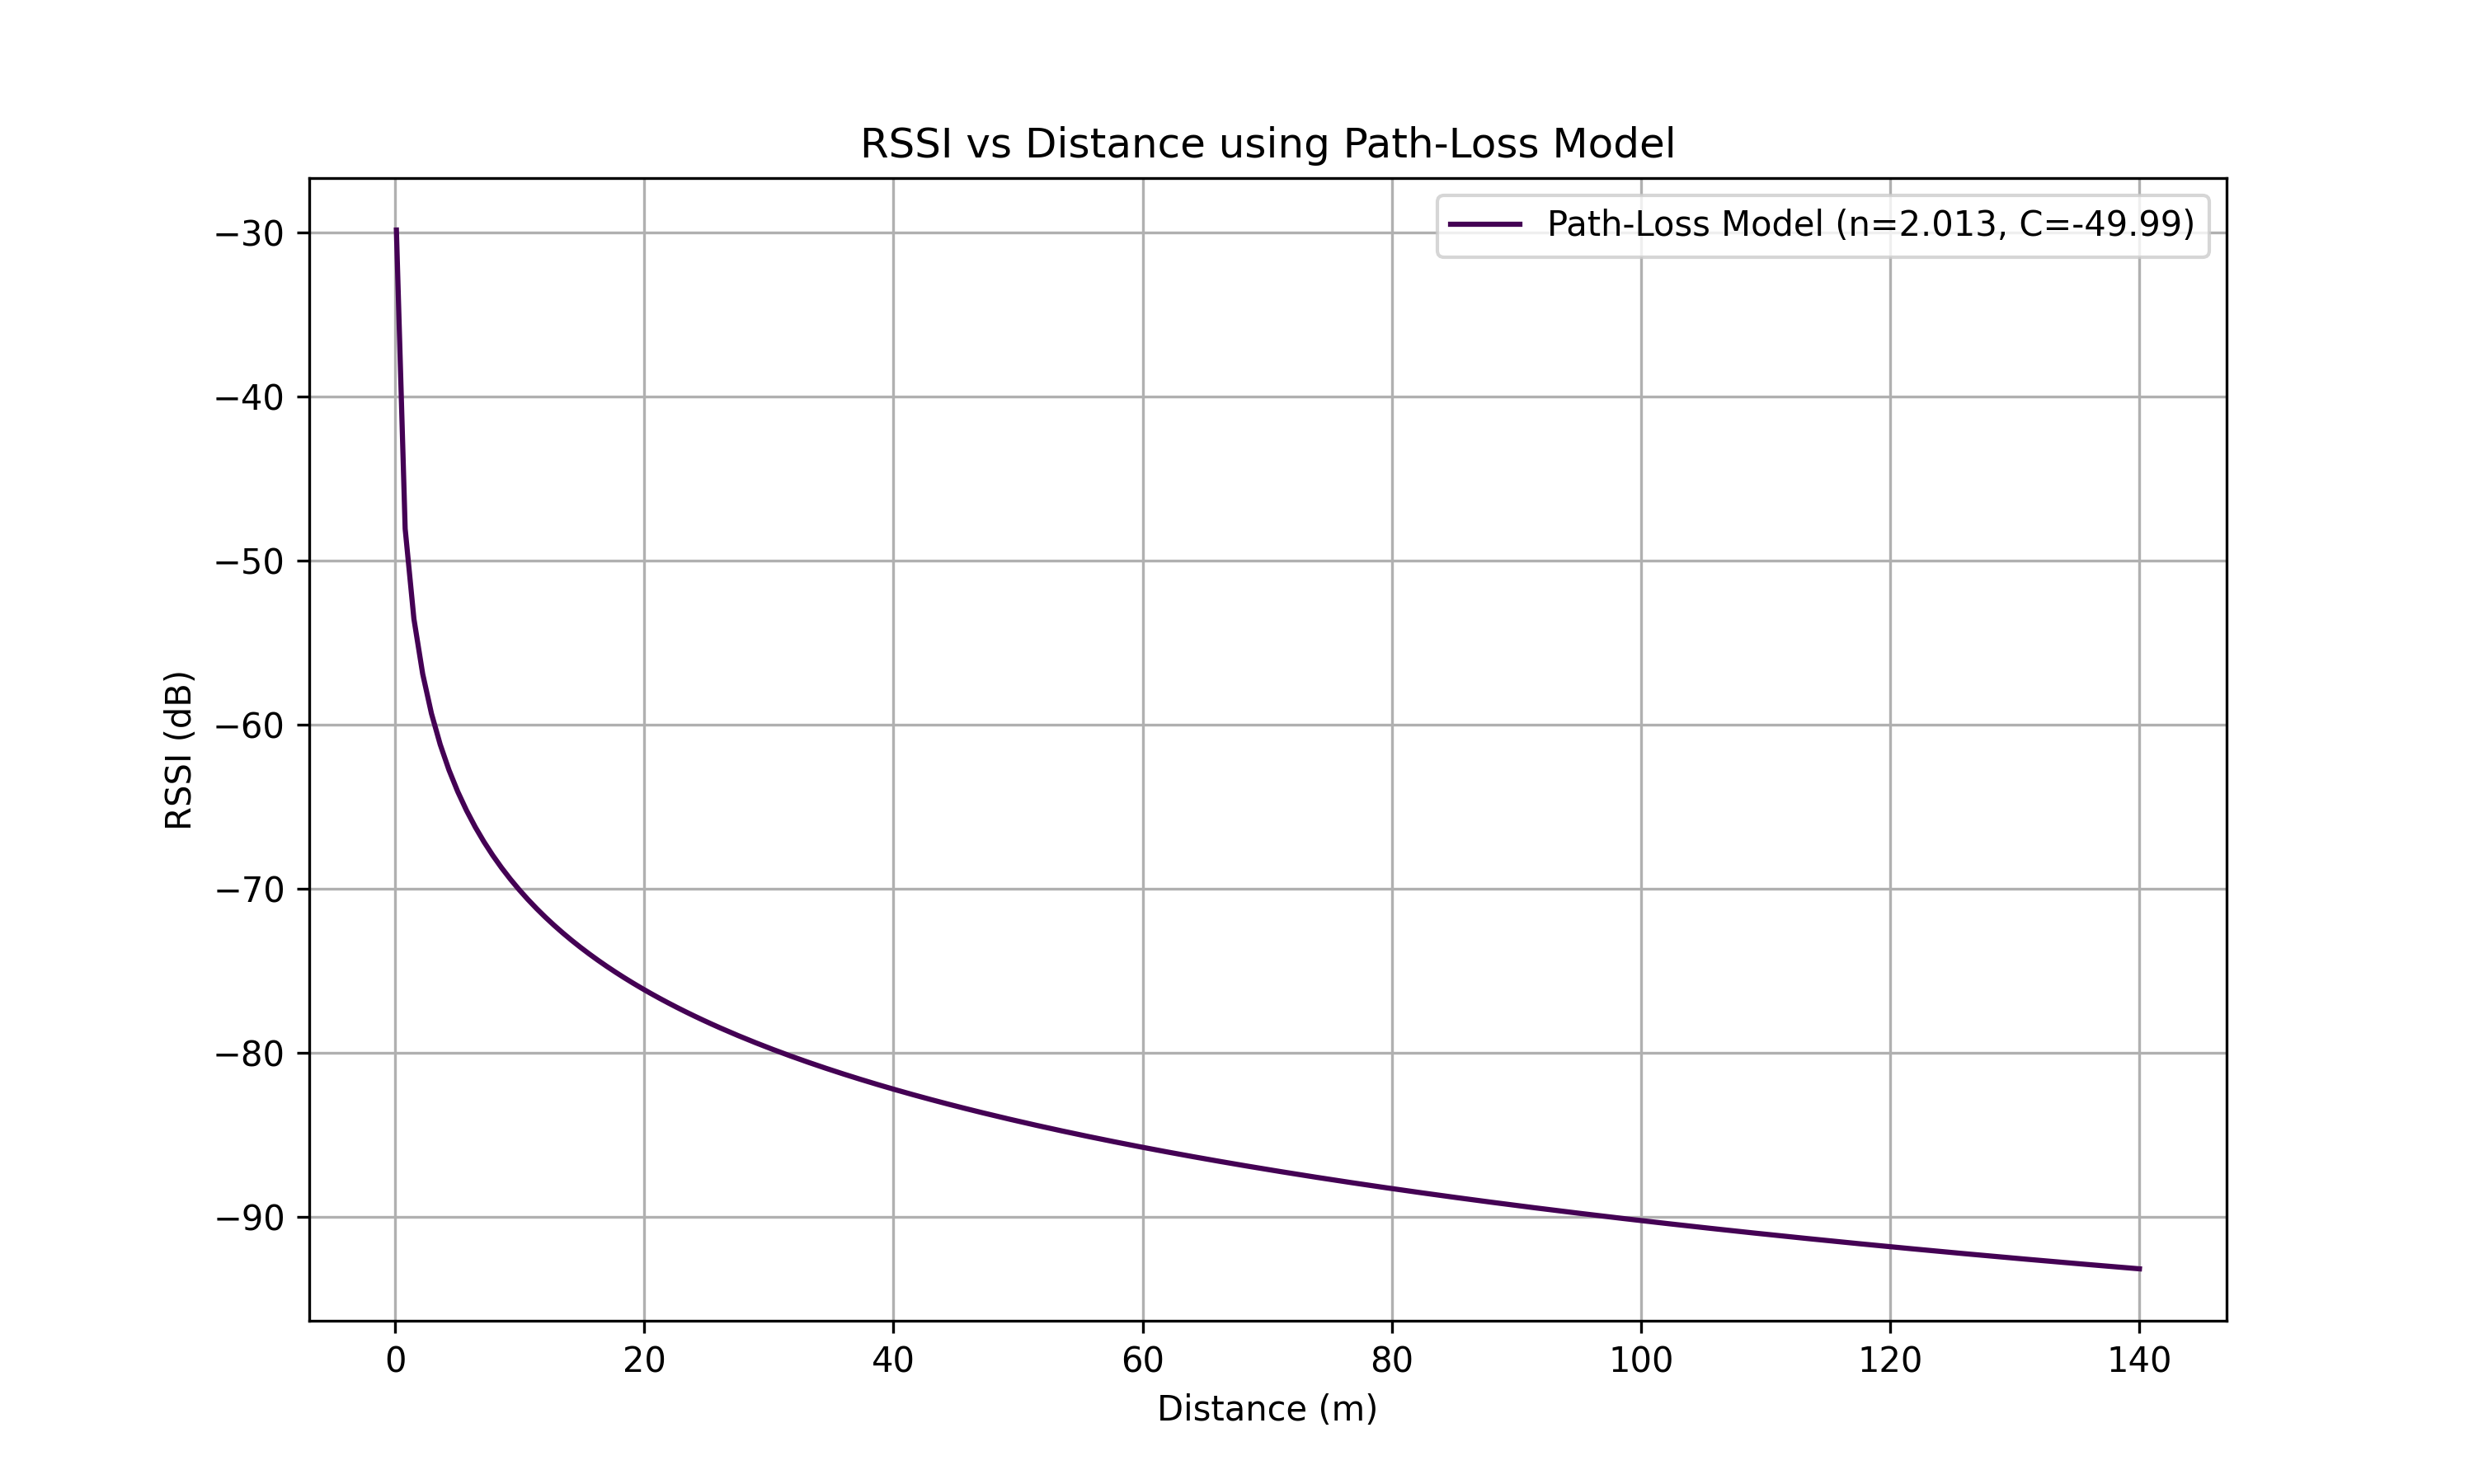
\includegraphics[width=0.8\textwidth]{images/rssi_distance.png}
    \caption{RSSI vs. Distance}
    \label{fig:rssi_distance}
\end{figure}